


%----------------------------------------------------------------------------------------

\newpage

\section[An Applied Knowledge Framework][Un Cadre de Connaissances Appliqué]{An Applied Knowledge Framework to Study Complex Systems}{Un Cadre de Connaissances Appliqué pour l'Etude des Systèmes Complexes}

\label{sec:knowledgeframework}


\bpar{
The complexity of knowledge production on complex systems is well-known, but there still lacks knowledge framework that would both account for a certain structure of knowledge production at an epistemological level and be directly applicable to the study and management of complex systems. We set a basis for such a framework, by first analyzing in detail a case study of the construction of a geographical theory of complex territorial systems, through mixed methods, namely qualitative interview analysis and quantitative citation network analysis. We can therethrough inductively build a framework that considers knowledge entreprises as perspectives, with co-evolving components within complementary knowledge domains. We finally discuss potential applications and developments.
}{
La complexité de la production de connaissance sur des systèmes complexes est bien connue, mais il n'existe toujours pas de cadre de connaissance qui rendrait à la fois compte d'une certaine structure de la production de connaissance à un niveau épistémologique et serait directement applicable à l'étude et au management des systèmes complexes. Nous posons ici les bases d'un tel cadre, en commençant par analyser en détail l'étude de cas de la construction d'une théorie géographique des systèmes territoriaux complexes, au travers de méthodes mixtes, plus précisément des analyses qualitatives d'entretiens et une analyse quantitative de réseau de citation. Nous pouvons par cela construire de manière inductive un cadre qui considère les entreprises de production de connaissance comme des perspectives, dont les composantes sont en co-évolution au sein de domaines de connaissances complémentaires. Nous discutons finalement des applications et développements potentiels.
}






\bpar{
The understanding of processes and conditions of scientific knowledge production are still mainly open questions, to which monuments of epistemology such as Kant's Critique of Pure Reason, and more recently Kuhn's study of ``the structure of scientific revolutions''~\cite{kuhn1970structure} or Feyerabend's advocacy for a diversity of viewpoints \cite{feyerabend1993against}, have brought elements of answer from a philosophical approach. A more empirical point of view was brought also recently with quantitative studies of science, in a way a \emph{quantitative epistemology} that goes far beyond rough bibliometric indicators~\cite{cronin2014beyond}. Contributions harnessing complexity, i.e. studying complex systems in a very broad sense, can be shown to have produced very diverse frameworks that can be counted as building bricks contributing to answers to the above high-level question. We will in the following use the term Knowledge Framework, for any such framework having an epistemological component tackling the question of nature of knowledge or knowledge production. To illustrate this, we can mention such frameworks in different domains, at different levels and with different purposes. For example, \cite{durantin2017disruptive} explores the potentialities of coupling engineering with design paradigms to enhance disruptive innovation. Also in Knowledge Management, using the constraint of innovation as an advantage to understand to complex nature of knowledge, \cite{carlile2004transferring} introduces knowledge domains boundaries and production processes. Also introducing a meta-framework, but in the field of system engineering, \cite{gemino2004framework} recommends to use grammars to compare Conceptual Modeling Techniques. Meta-modeling frameworks can also be understood as Knowledge Frameworks. \cite{cottineau2015modular} describes a multi-modeling framework to test hypotheses in simulation of socio-technical complex systems. \cite{golden2012modeling} postulates a unified formulation of systems, including necessarily different types of knowledge on a system on its different description components.
}{
La compréhension des processus et des conditions de production de la connaissance scientifique est une question toujours globalement ouverte, à laquelle des monuments de l'épistémologie comme la Critique de la Raison Pure de Kant, ou plus récemment l'étude par Kuhn de la ``structure des révolutions scientifiques''~\cite{kuhn1970structure} ou le positionnement de Feyerabend pour une diversité des approches~\cite{feyerabend1993against}, ont apporté des éléments de réponse d'un point de vue philosophique. Un matériau plus empirique a été apporté également récemment avec les analyses quantitatives de la science, dans un sens une \emph{épistémologie quantitative} qui va bien plus loin que des indicateurs bibliométriques purs~\cite{cronin2014beyond}. Les contributions s'intéressant à la complexité, c'est à dire étudiant des systèmes complexes en un sens très large, peuvent témoigner de la production de cadre de travail très divers qui peuvent être vus comme des éléments élémentaires de réponse à la question à un autre niveau ci-dessus. Nous utiliserons par la suite le terme \emph{Cadre de Connaissances}, pour tout cadre tel ayant une composante épistémologique s'intéressant à la nature de la connaissance et à sa production. Pour illustrer, nous pouvons mentionner de tels cadres dans différents domaines, à différents niveaux, et avec des but différents. Par exemple, \cite{durantin2017disruptive} explore les potentialités de coupler l'ingénierie avec des paradigmes du design to encourager l'innovation disruptive. Toujours en Gestion de Connaissances, utilisant la contrainte de l'innovation comme un avantage pour appréhender la nature complexe de la connaissance, \cite{carlile2004transferring} introduit les notions de frontières des domaines de connaissance et de processus de production. Introduisant également un framework meta, mais dans le champ de l'ingénierie des systèmes, \cite{gemino2004framework} recommande l'utilisation de grammaires pour comparer les techniques de Modélisation Conceptuelle. Les cadres de meta-modélisation peuvent aussi être compris comme des cadres de connaissance. \cite{cottineau2015modular} décrit un cadre de multi-modélisation pour le test d'hypothèses dans la simulation des systèmes complexes socio-techniques. \cite{golden2012modeling} postule une formulation unifiée de la notion de système, ce qui inclut nécessairement différents types de connaissance sur un système correspondant à la description de ses différents composants.
}
 
 
\bpar{
A possible explanation for this richness is the fundamental reflexive nature of the study of Complex Systems: because of the higher choice in methodology and what aspects of the system to put emphasis on, a significant part of a modeling or design entreprise is an investigation at a meta-level.  Furthermore, studies of knowledge production are mainly rooted in complexity, implying a reflexive nature of theories accounting knowledge on complexity, as Hofstadter had well highlighted in \cite{hofstadter1980godel} by noticing the importance of ``strange loops'', i.e. feedback loops allowing reflexivity such as a theory applying to itself, in what constitutes intelligence and the mind. Artificial intelligence is indeed a crucial field regarding our issues, as its progresses imply a finer understanding of the nature of knowledge. \cite{2017arXiv170401407M} introduces a meta-framework for a general typology of approaches in Artificial Intelligence, what is a Knowledge Framework not in the proper sense but in a specific applied case.
}{
Une explication possible pour une telle richesse est la nature fondamentalement réflexive de l'étude des Systèmes Complexes : à cause du choix plus grand pour la méthodologie et sur quels aspects du système mettre l'emphase, une partie significative d'une entreprise de modélisation ou de design est une exploration à un niveau meta. De plus, les études de la production de connaissance sont profondément ancrées dans la complexité, comme Hofstadter a bien souligné dans \cite{hofstadter1980godel} en rappelant l'existence de ``boucles étranges'', c'est à dire de boucles de rétroaction permettant la reflexivité comme une théorie s'appliquant à elle-même, dans ce qui constitue l'intelligence et l'esprit. L'intelligence artificielle est de fait un champ crucial au regard de nos reflexions, comme ses progrès impliquent une compréhension plus fine de la nature de la connaissance. \cite{2017arXiv170401407M} introduit un meta-cadre pour une typologie générale des approches en intelligence artificielle, ce qui correspond à un cadre de connaissance non au sens propre mais dans un cas particulier d'application.
}


\bpar{
The level of frameworks described above may be very general but is conditioned to a certain field or discipline, and to a certain approach or methodology. There exists to our knowledge no framework realizing a difficult exercise, that is to capture a certain structure of knowledge production at an epistemological knowledge, but conjointly is thought in a very applied perspective, with direct consequence in the design and management of complex systems. The contribution of this paper attempts to set a basis for a Knowledge Framework realizing this in the case of Complex Systems. To perform that, we postulate that the tension between these two contradictory objective is an asset to avoid on one side an impossible overarching generality and on the other side a too restraining domain-specific specificity. Based on the idea of complementary Knowledge Domains introduced by~\cite{livet2010}, its central aspect is a cognitive approach to science inducing co-evolutive processes of knowledge domains and their carriers. A first sketch of this framework was presented by~\cite{raimbault:halshs-01505084}, in the specific case of complex territorial systems as studied by theoretical and quantitative geography. We choose to introduce it here with an inductive approach, i.e. starting from a concrete case study that has mainly inspired the construction of the framework to end with its generic description.
}{
Le niveau des cadres présentés ci-dessus peut être très général mais reste conditionné à un certain champ ou discipline, et à une certaine approche ou méthodologie. Il n'existe à notre connaissance pas de cadre réalisant un exercice difficile, qui est de capturer une certaine structure de production de la connaissance à un niveau épistémologique, mais qui est conjointement pensée dans une perspective très appliquée, avec des conséquences directes pour la conception et la gestion de systèmes complexes. La contribution de cette partie propose de poser les bases pour un cadre réalisant cela dans le cas des Systèmes Complexes. Pour y parvenir, nous partons du postulat que la tension entre ces deux objectifs contradictoires est un atout pour éviter d'une part une généralité globale impossible et d'autre part une spécificité due à un domaine qui serait trop restrictive. En se basant sur l'idée des domaines de connaissance introduite par~\cite{livet2010}, son aspect central est une approche cognitive de la science qui implique des processus de co-evolution entre les domaines de connaissance et leur supports. Une première ébauche de ce cadre a été présentée par~\cite{raimbault:halshs-01505084}, dans le cas particulier des systèmes complexes territoriaux comme étudiés par la géographie théorique et quantitative. Nous proposons de l'introduire ici par une démarche inductive, c'est à dire en partant d'une étude de cas concrète qui a largement inspiré la construction du cadre, pour finir avec sa description générique.
}


\bpar{
The rest of the paper is organized as follows : the next section develops case studies, more precisely a detailed study of a geographical theory of complex urban systems, and a short example from engineering to illustrate the transferability of concepts. The third section specifies the definitions and formulates the epistemological framework. We finally discuss issues on applicability, and potential developments such as a mathematical version of the framework.
}{
%La suite de cette section est organisée de la façon suivante : 
}



%%%%%%%%%%%%%%%%
\subsection{Case Studies}{Etude de cas}
%%%%%%%%%%%%%%%%


%%%%%%%%%%%%%%%%
\subsubsection{Genesis of the Evolutive Urban Theory}{Genèse de la Théorie Evolutive Urbaine}



\bpar{
The first case study relates the construction of the \emph{Evolutive Urban Theory}, a geographical theory considering territorial systems from a complexity perspective, that have been developed for around 20 years. We analyse its genesis using mixed methods, namely semi-directed interviews with main contributors, and quantitative bibliometric analysis of main publications. Interviews were done following methodological standards \cite{legavre1996neutralite} to ensure a limited interference of the interviewer's experiences but not make it fully disappear to ensure a precise context enhancing the fluency of the interviewed. We use here interviews\footnote{Both have a length of around 1h. Sound and transcript text are available under a CC Licence at \texttt{https://github.com/JusteRaimbault/Interviews}~\cite{raimbault2017entretiens}. Interviews are in French and translations here are done by the author.} with Pr. D. Pumain who introduced and developed mainly the theory, and Dr. R. Reuillon, whose research on intensive and distributed computation and model exploration has been a cornerstone of latest developments.
}{
La première étude de cas rappelle la construction de la \emph{Théorie Evolutive Urbaine}\footnote{l'ambiguïté de l'adjectif \emph{évolutive} fait gagner la théorie en subtilité, puisqu'il s'applique aussi bien au sens premier c'est à dire aux entités urbaines étudiées, mais aussi à un sens meta à la théorie elle-même, ce qui confirme un certain niveau de réflexivité de la théorie qui est essentiel comme développé en~\ref{sec:epistemology}. Pour traduire le terme en anglais, il a été choisi ``Evolutionary Urban Theory'' par \cite{pumain2006evolutionary}, mais ``Evolutive Urban Theory'' convient aussi, mais il semble dans tous les cas difficile de transférer l'ambiguïté lors de la traduction.}, une théorie géographique qui considère les systèmes territoriaux par une perspective complexe, développée depuis une vingtaine d'années environ. Nous étudions sa genèse par l'utilisation de méthodes mixtes, c'est à dire à la fois des interviews semi-dirigées avec des contributeurs principaux, et une analyse bibliométrique quantitative des publications principales. Les interviews ont été menées en suivant les standards méthodologiques classiques~\cite{legavre1996neutralite} pour assurer une interférence limitée des expérience de l'interviewer, mais sans le faire disparaitre complètement afin de permettre un contexte précis favorable à la fluidité de l'interviewé. Nous utilisons ici des interviews\footnote{Toutes les deux d'une durée environ une heure. Le son et les transcripts sont disponibles sous une Licence CC à \texttt{https://github.com/JusteRaimbault/Interviews}~\cite{raimbault2017entretiens}. Les interviews sont en français et la traduction anglaise des passages cités dans l'article original est assurée par l'auteur.} avec Pr. D. Pumain qui a introduit et développé majoritairement la théorie, et Dr. R. Reuillon, dont la recherche sur le calcul intensif et distribué et l'exploration de modèles a été une pierre d'angle des développements les plus récents.
}


\bpar{
Let first give an overview of its content. This theory was first introduced in~\cite{pumain1997pour} which argues for a dynamical vision of city systems, in which self-organization is key. Cities are interdependent evolutive spatial entities whose interrelations produces the macroscopic behavior at the scale of city system. The city system is also described as a network of city what emphasizes its view as a complex system. Each city is itself a complex system in the spirit of~\cite{berry1964cities}, the multi-scale aspect being essential in this theory, since microscopic agents convey system evolution processus through complex feedbacks between scales. The positioning within Complex System Sciences was later confirmed~\cite{pumain2003approche}. It was shown that this theory provide an interpretation for the origin of pervasive scaling laws, resulting from the diffusion of innovation cycles between cities~\cite{pumain2006evolutionary}. The aspect of resilience of system of cities, induced by the adaptive character of these complex systems, implies that cities are drivers and adapters of social change~\cite{pumain2010theorie}. Finally, path dependance yield non-ergodicity within these systems, making ``universal'' interpretations of scaling laws difficultly compatible with evolutive urban theory~\cite{pumain2012urban}. The construction of models of urban systems has been a key component for the theory, starting with the first Simpop model~\cite{sanders1997simpop}. Later example include for example the Simpop2 model, an agent-based model taking into account economic processes, that simulates growth patterns on long time scales for Europe and the United States~\cite{doi:10.1177/0042098010377366}. The latest accomplishment of the evolutive theory relies in the output of the ERC project GeoDivercity, presented in~\cite{pumain2017urban}, that include both advanced technical (software OpenMole\footnote{http://openmole.org/}~\cite{reuillon2013openmole}), thematic (knowledge from SimpopLocal~\cite{schmitt2014modelisation} and Marius models~\cite{cottineau2014evolution}) and methodological (incremental modeling~\cite{cottineau2015incremental}) progresses.
}{
Pour commencer il est important de se rappeler un aperçu rapide du contenu de la théorie évolutive. Pour cela, consulter le deuxième pilier de notre théorie géographique en~\ref{sec:theory}, qui en donne la substantifique moelle.
}


\bpar{
The striking feature in the construction of all this is the balance between the different \emph{types} of knowledge, of which a typology will be the starting point of our construction. The relation between theoretical considerations and empirical cases studies is fundamental. Indeed, the seminal article \cite{pumain1997pour} is already positioned as an ``advocacy for a less ambitious theory, but that does not neglects the back-and-forth with observation''\footnote{page 2, trad. author}. We shall now turn to interviews to better understand the implications of the intrication of types of knowledge. D. Pumain traces back germinal ideas back to her graduate student work in 1968, when ``everything started with a question of data''. The interest for cities, and \emph{change in cities}, was driven by the availability of a refined migration flow dataset at different dates. Also rapidly, ``[they] were frustrated that methods were missing'', but the access to the computation center (\emph{technical tool}) allowed the test of newly introduced methods and models, linked to the Prigogine approach to complexity. Methods were however still limited to grasp the heterogeneity of spatial interactions. A progressively specified need and a chance encounter, with ``a lady working on neural networks and agent-based modeling at the Sorbonne'', led to a bifurcation and a new level of interaction between modeling, theory and empirical knowledge: in 1997, two seminal articles, one stating the theoretical basis and the other introducing the first Simpop model, were published. From this point, it was clear that all modeling entreprise was conditioned to empirical knowledge of geographical case studies and theoretical assumptions to test. Methods and technical tools took also a necessary role, when specific model exploration methods were developed together with the Software OpenMole. R. Reuillon relates that a qualitative shift of knowledge was rapidly made possible when systematic model exploration methods were introduced to understand the behavior of the SimpopLocal model. Initially, geographers were not sure if the model worked at all, in the sense that it produced expected stylized facts such as the emergence of hierarchy in a system of cities. Satisfying trajectories were found for some parameter values through genetic algorithm calibration, with distributed computation on grid~\cite{schmitt2014half}. The existence of multiple candidate solutions for parameter values is a barrier for concrete questions of necessity or sufficiency of a given mechanism of the agent-based model. This need, coming from the domain of empirical and theoretical geographical knowledge, led to the design of a specific algorithm the calibration profile, which is a methodological advance in model exploration~\cite{reuillon2015}. This virtuous circle was continued with the Marius model family~\cite{cottineau2014evolution} and the Parameter Space Exploration algorithm~\cite{10.1371/journal.pone.0138212}. R. Reuillon evaluates its impact from a Computer Scientist point of view: ``I'm not sure if [geographers] were immediately conscious of the amplitude of the result, that was really heavy, people working with us directly saw it.'' This positive vision is confirmed by D. Pumain, who highlights the benefits of these new methods for geographical knowledge, and that it was the first time that research led to publications at the edge of knowledge both in geography and computer science.
}{
La caractéristique frappante dans cette construction est l'équilibre entre les différents \emph{types} de connaissance, desquelles une typologie sera le point de départ de notre construction. La relation entre les considérations théoriques et les cas d'étude empiriques est fondamental. En effet l'article séminal \cite{pumain1997pour} est déjà positionné comme ``un plaidoyer pour une théorie [...] moins ambitieuse, mais qui ne néglige pas les aller-retours avec l'observation''. Nous pouvons maintenant nous tourner vers les entretiens pour mieux comprendre les implications de l'intrication des différents types de connaissance. D. Pumain retrace les idées germinales à son travail de maîtrise en 1968, quand ``tout à commencé avec une question de données''. L'intérêt pour les villes, et pour le \emph{changement dans les villes}, a été conduit par la disponibilité d'un jeu de données raffiné sur les flux migratoires à différentes dates. Egalement rapidement, est venue ``la frustration des méthodes qui manquaient'', mais l'accès au centre de calcul (\emph{outil technique}) a permis le test de méthodes et modèles nouvellement introduits, liés à l'approche de la complexité par Prigogine. Les méthodes restaient toutefois limitées pour capturer l'hétérogénéité des interactions spatiales. Un besoin progressivement spécifié et une rencontre fortuite, avec ``une dame qui travaillait sur les réseaux de neurones et les modèles agents à la Sorbonne'', a conduit à une bifurcation et un nouveau niveau d'interaction entre modèles, théorie et connaissance empirique : en 1997, deux articles séminaux, l'un donnant la base théorique, l'autre introduisant le premier modèle Simpop, étaient publiés simultanément. A partir de ce point, il était clair que toute entreprise de modélisation était conditionnée à une connaissance empirique de cas d'étude géographiques et à des hypothèses théoriques à tester. Les méthodes et les outils techniques ont alors pris aussi un rôle nécessaire, avec des méthodes d'exploration de modèles spécifiques développées avec le logiciel OpenMole. R. Reuillon raconte qu'un saut qualitatif de connaissances a été rendu rapidement possible quand les méthodes d'exploration systématiques ont été introduites pour comprendre le comportement du modèle SimpopLocal. A la base, les géographes n'étaient pas sûr si le modèle fonctionnait seulement, dans le sens où il produisait les faits stylisés attendus comme l'émergence de la hiérarchie d'un système de villes. Des trajectoires satisfaisantes ont été trouvées par l'utilisation d'algorithmes génétiques de calibration, en calcul distribué sur grille~\cite{schmitt2014half}. L'existence de multiples solution équivalentes pour les valeurs des paramètres est une barrière pour des question concrètes de nécessité ou suffisance d'un mécanisme donné du modèle agent. Ce besoin, venant du domaine de la connaissance empirique et théorique géographique, a mené à la conception d'un algorithme spécifique : le Calibration Profile, qui est une avancée méthodologique dans l'exploration de modèles~\cite{reuillon2015}. Ce cercle vertueux a été continué avec la famille de modèles Marius~\cite{cottineau2014evolution} et l'algorithme Parameter Space Exploration~\cite{10.1371/journal.pone.0138212}. R. Reuillon évalue son impact du point de vue d'un informaticien : ``Je ne suis pas sûr si les géographes étaient immédiatement conscients de la portée du résulat, c'était du lourd, les gens qui bossaient avec nous l'ont directement vu.'' Cette vision positive est confirmée par D. Pumain, qui souligne les bénéfices de ces nouvelles méthodes pour la connaissance Géographique, et que c'était la première fois qu'une recherche menait à des publications à la frontière de la connaissance à la fois en géographie et en informatique.
}


\bpar{
Taking a step back, emerges a typology of domains in which knowledge was created but also necessary for the other domains in the genesis of the Evolutive Urban Theory. The collection of data and construction of datasets is a first requirement for any further knowledge. From data are extracted empirical stylized facts, from which are induced theoretical hypotheses. Theory can then be tested for falsification, in the empirical domain but also through models, for example by doing targeted experiments in models of simulation. New methods are developed to better explore them. Tools are crucial at each step, to implement model, do data mining for example or collect and format data for example. The previous analysis reveals how these domains are interdependent, are in a sense \emph{co-evolutive}.
}{
En prenant du recul, émerge une typologie de domaines dans laquelle de la connaissance a été créée mais également nécessaire pour les autres domaines dans la genèse de la Théorie Evolutive Urbaine. La récolte des données et la construction de jeux de données est un premier pré-requis pour toute connaissance supplémentaire. A partir des données on extrait des faits stylisés empiriques, desquels sont déduits des hypothèses théoriques. La Théorie peut être testée pour falsification, dans le domaine empirique mais aussi par les modèles, par exemple par des expériences ciblées dans les modèles de simulation. De nouvelles méthodes sont alors développées pour mieux les explorer. Les outils sont cruciaux à chaque étape, pour implémenter un modèle, faire de la fouille de données ou collecter et formater les données par exemple. L'analyse précédente montre comment ces domaines sont interdépendants, et sont dans un sens \emph{co-évolutifs}.
}


\bpar{
We back up now this qualitative analysis with a modest quantitative bibliometric analysis. The idea is to investigate the structure of the core citation network of main publications constructing the Evolutive Urban Theory. We construct the citation network as described in Fig.~\ref{fig:citnw}, by using the data collection tool provided by~\cite{raimbault2016indirect}\footnote{all code and data are available at \\\texttt{https://github.com/JusteRaimbault/CityNetwork/tree/master/Models/QuantEpistemo}}. Starting from the two seminal publications \cite{pumain1997pour} and \cite{sanders1997simpop}, the backward citation network is obtained at depth 2 (references citing these initial references, and the ones citing the citing), with filtering for the first step on authors to have at least one main contributor of the Theory (that we take as \emph{Pumain}, \emph{Sanders} and \emph{Bretagnolle}, according to the full Pumain's interview). We remove nodes of degree 1, to have the core structure only of the ego network. Note that we do not have missing links between nodes at the first level, because all citing links were retrieved. Network has a density of 0.019, what is rather high for a citation network, and the signature of a high level of dependency between publications. Starting from two separate nodes, we could have in theory distinct connected components, but as expected the network has only one because both aspects are strongly interconnected. To analyse the structure in a finer way, we detect communities using Louvain clustering algorithm, and evaluate the directed modularity of the partition as described by \cite{nicosia2009extending}. We show in Fig.~\ref{fig:citnw} a visualization of the network. We obtain 7 communities with a modularity value of 0.39. To ensure the significance of modularity, we proceed to Monte Carlo simulations and randomize citation links 100 times, computing each time the modularity of communities within the randomized network. We obtain an average directed modularity of $\bar{m} = 0.002 \pm 0.015$, making the modularity of the real network highly significant (more than 200 standard deviations). We analyse the content of communities by looking at publications of the first level. We find that communities are roughly consistent with the typology of domains: one on methods, three on spatio-temporal modeling of urban systems that mixes empirical and modeling, one conceptual, one on Simpop models, and a last on scaling laws that is fully empirical. Data papers are not yet current practice in geography and specific papers tackling the Data domain cant be found in the network. An increased citation rate between papers of the same domain could be expected because of the scientific standard to always situate a contribution regarding similar works. The significant value of modularity confirms that domains are consistent regarding an certain endogenous structure of knowledge production.
}{
Nous supportons cette analyse qualitative par une analyse quantitative bibliométrique modeste. L'idée est d'étudier la structure du coeur du réseau de citations des publications principales construisant la Théorie Evolutive Urbaine. Nous construisons le réseau de citations comme décrit en Fig.~\ref{fig:citnw}, en utilisant l'outil de collection de données fournit par~\cite{raimbault2016indirect}\footnote{l'ensemble du code et des données pour cette analyse sont disponibles à \\\texttt{https://github.com/JusteRaimbault/CityNetwork/tree/master/Models/QuantEpistemo}}. Partant des deux publications séminales \cite{pumain1997pour} et \cite{sanders1997simpop}, le réseau de citation inverse est obtenu à profondeur 2 (les références citant ces références initiales, et celles citant les citantes), en filtrant à la première étape sur les auteurs pour avoir au moins un des principaux contributeurs de la théorie (que nous prenons comme \emph{Pumain}, \emph{Sanders} et \emph{Bretagnolle}, en accord avec l'entretien avec D. Pumain). Les noeuds de degré 1 sont supprimés, pour obtenir uniquement le coeur du réseau d'ego. On peut noter qu'il ne manque pas de lien entre les noeuds du premier niveau, puisque tous les liens citants ont été récupérés. Le réseau a une densité de 0.019, ce qui est plutôt élevé pour un réseau de citation, et la signature d'un haut niveau de dépendance entre les publications. En partant de deux noeuds distincts, nous aurions pu avoir en théorie des composantes connexes distinctes, mais comme attendu le réseau n'en a qu'une de par la nature fortement interconnectée des deux aspects. Pour analyser la structure de manière plus fine, nous détectons les communautés en utilisant l'algorithme de clustering de Louvain, et évaluons la modularité dirigée de la partition comme donnée par \cite{nicosia2009extending}. Nous montrons en Fig.~\ref{fig:fig:knowledgeframework:citnw} une visualisation du réseau. Nous obtenons 7 communautés avec une valeur de modularité de 0.39. Pour assurer que cette valeur est significative, nous procédons à des simulations de Monte Carlo et distribuons de manière aléatoire les liens de citation 100 fois, en calculant à chaque fois la modularité des communautés dans le réseau aléatoire. Nous obtenons une modularité moyenne dirigée de $\bar{m} = 0.002 \pm 0.015$, rendant la modularité du réseau réel hautement significative (plus de 200 déviations standard). Nous analysons le contenu des communautés en examinant leur publications du premier niveau. Nous trouvons que les communautés sont globalement cohérentes avec les typologie des domaines : une pour les méthodes, trois sur la modélisation spatio-temporelle des systèmes urbains qui mélange empirique et modélisation, une conceptuelle, une sur les modèles Simpop, et une dernière sur les lois d'échelle qui est complètement empirique. Les \emph{Data Papers} ne sont pas encore une pratique courante en géographie et des articles spécifiques au domaine des données ne peuvent être trouvés dans le réseau. Un taux de citation accru entre papiers du meme domaine est dans tous les cas attendu à cause du standard scientifique de toujours situer une contribution au regard des travaux similaires. La valeur significative de la modularité confirme que les domaines sont cohérents au regard d'une certaine structure endogène de la production de connaissance.
}

% content of communities :
%  (1) METHODS SimpopLocal calib, modular Framwork
%  (5) The organization of urban systems, Time and space scales for measuring urban growth, Space-time contraction and the dynamics of urban systems
%  (7) La ville et la croissance urbaine dans l'espace-temps, Les modèles d'auto-organisation et le changement urbain, Villes, agents et acteurs en géographie
%  (3) Cognition and decision in multi-agent modeling of spatial entities at different geographical scales, Long-term dynamics of European towns and cities: towards a spatial model of urban growth, Knowledge-based simulation of settlement systems, The socio-spatial dynamics of systems of cities and innovation processes: a multi-level model, Villes et systèmes de villes dans l'économie, Urban research and complexity
%  (4) CONCEPTUEL Une approche de la complexité en géographie" " Une théorie géographique des villes" 
%  (2) SIMPOP MODELS  Intelligence artificielle et agents collectifs: le modèle EUROSIM, The future of urban systems: exploratory models, SIMPOP: a multiagent system for the study of urbanism, Agonistic pluralism and stakeholder engagement, Les modèles agent en géographie urbaine, Modélographie multi-agents de la simulation des interactions sociétés-environnement et de l'émergence des villes, La mesure de l'urbanisation aux États-Unis, des premiers comptoirs coloniaux aux Metropolitan Areas (1790-2000), Multi-agent system modelling for urban systems: The series of SIMPOP models"  
%  (6) SCALING LAWS City size distributions and metropolisation, Alternative explanations of hierarchical differentiation in urban systems, Systèmes de villes et niveaux d'organisation


%%%%%%%%%%%%%%%%
\begin{figure}[h!]
\hspace{-4cm}
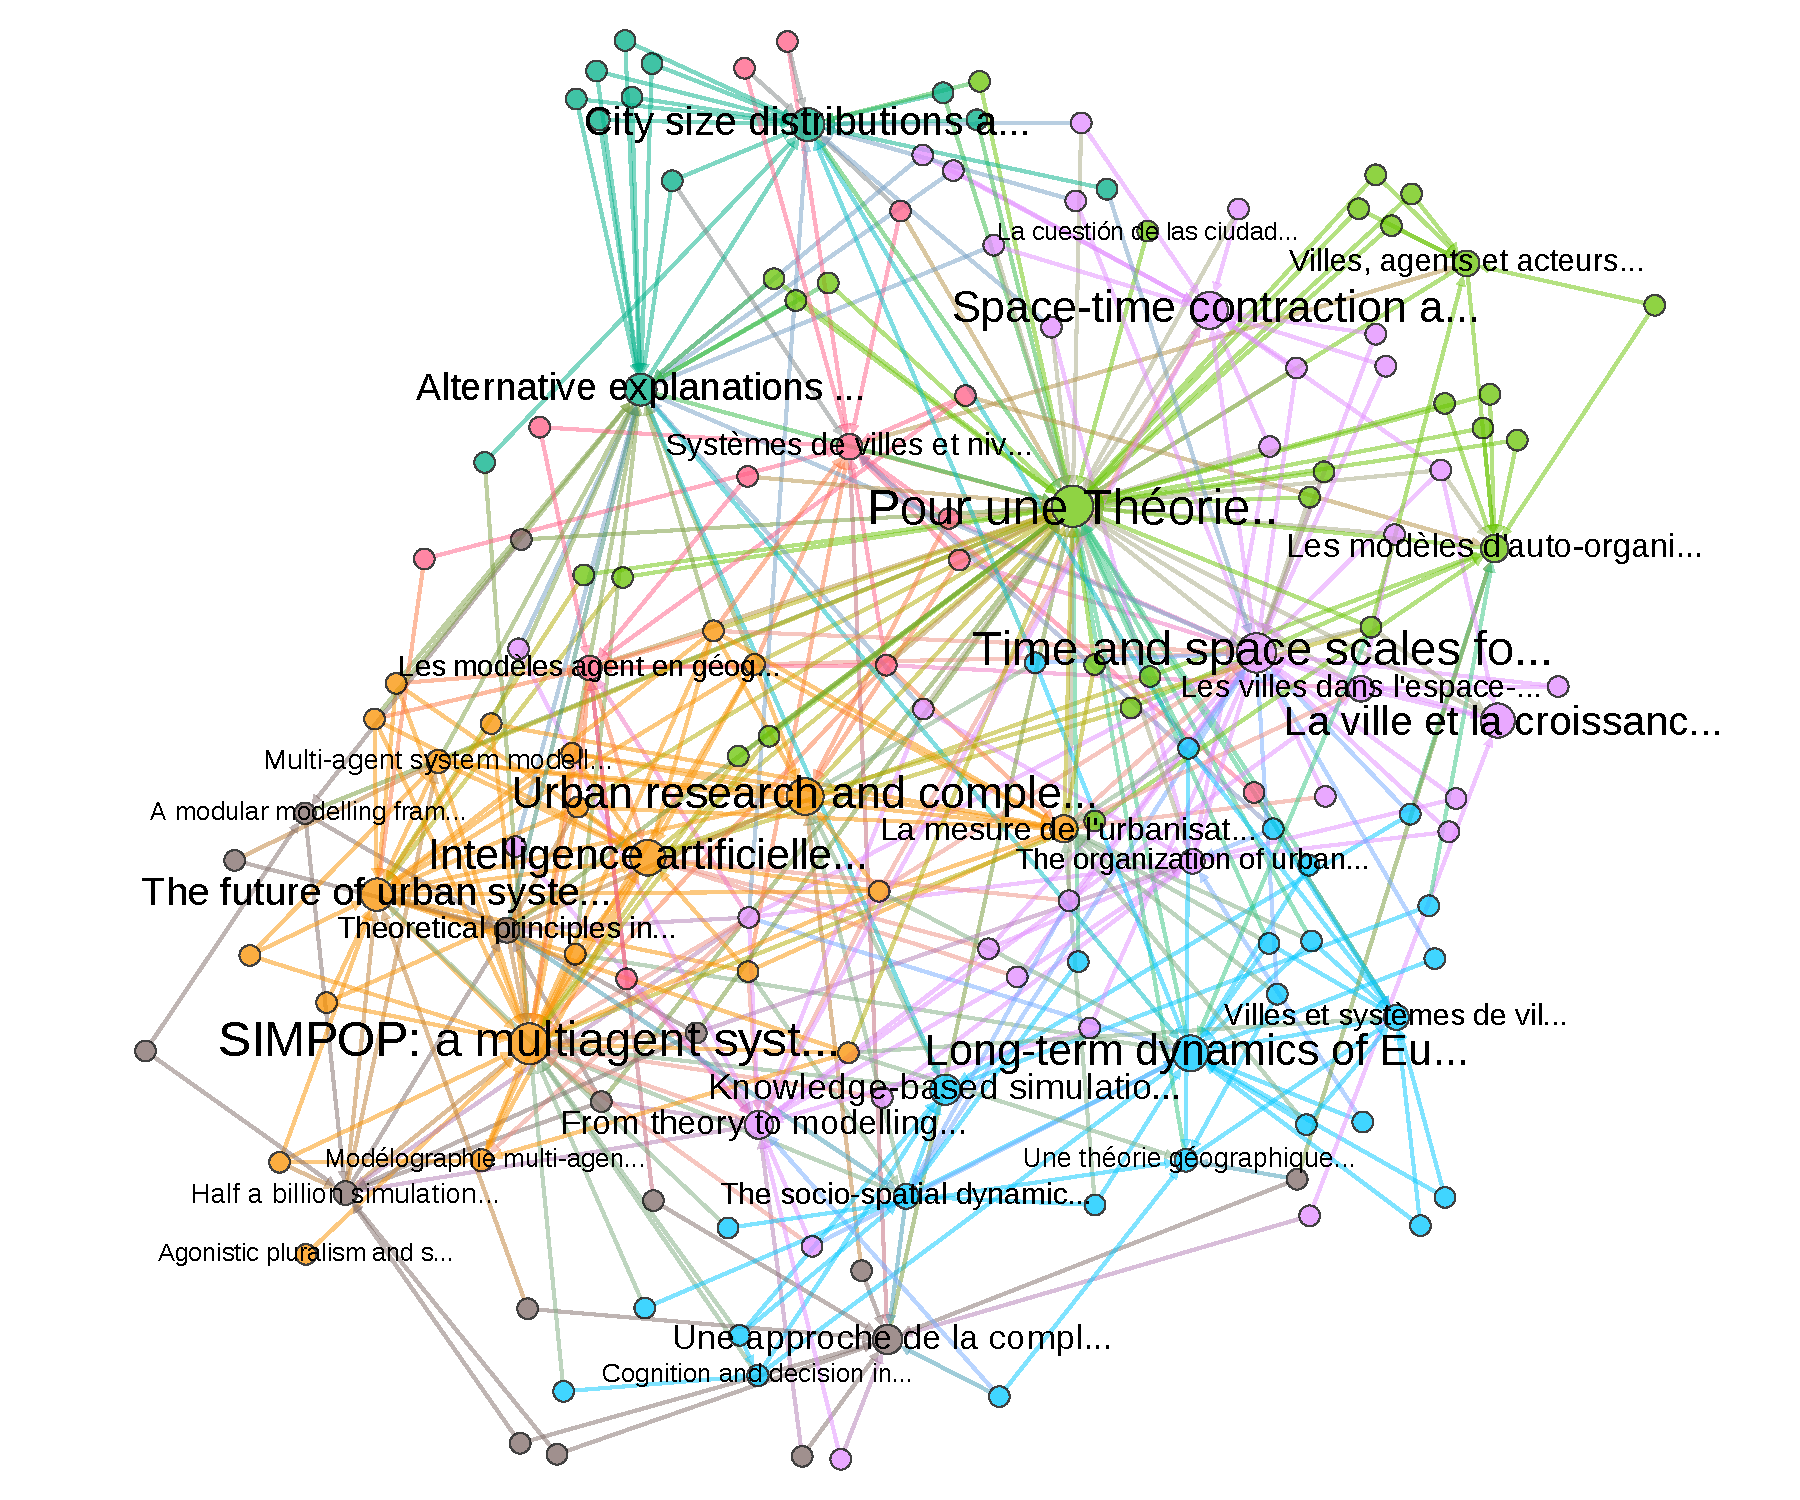
\includegraphics[width=1.5\textwidth]{Figures/KnowledgeFramework/core}
\caption[Citation Network of main publications of Evolutive Urban Theory][Réseau de citations de la Théorie Evolutive Urbaine]{\textbf{Citation Network of main publications of Evolutive Urban Theory.} The network is constructed the following way: starting from the two seminal publications~\cite{pumain1997pour} and \cite{sanders1997simpop}, we get citing publications, filter conditionally to one of the main contributors, get again citing publications and filter. Nodes are publications ($\left|V\right|=155$), the size corresponding to eigenvector centrality, and edges are directed citation links ($\left|E\right|=449$). Colors are communities obtained with Louvain clustering algorithm (7 communities, modularity 0.39).}{\textbf{Réseau de citations des publications principales de la Théorie Evolutive Urbaine.} Le réseau est construit de la manière suivante : à partir des deux publication séminales \cite{pumain1997pour} and \cite{sanders1997simpop}, nous récupérons les publications les citant, filtrons sous la condition d'un des contributeurs principaux appartenant aux auteurs, récupérons encore les publications citantes et filtrons. Les noeuds sont les publications ($\left|V\right|=155$), leur taille correspondant à la centralité de vecteur propre, et les liens sont les liens de citation dirigés ($\left|E\right|=449$). La couleur donne les communautés obtenues par l'algorithme de clustering de Louvain (7 communautés, modularité 0.39).}
\label{fig:fig:knowledgeframework:citnw}
\end{figure}
%%%%%%%%%%%%%%%%




%%%%%%%%%%%%%%%%
\subsubsection{Engineering the Metropolitan}{Ingéniérie}


\bpar{
After the glance on domains of knowledge extracted in the previous case study, we propose to take the corresponding point of view on a rather different example more related to technology and engineering. We interpret thus issues of engineering related to Parisian metropolitan system through this prism of Knowledge Domains. Taking the example of the progressive automatization of line 1, considered widely as a technical achievement, several integrated empirical and modeling studies were preliminary conducted~\cite{belmonte2008automatisation}. The use and adaptation of particular methods such as agent-based modeling is crucial for the development of innovative autonomous transportation~\cite{balbo2016positionnement}. In this engineering problem, some technical solutions such as platform doors may be seen as tools that also evolve, and are necessary for a new conceptual approach (\emph{automatic transportation}) to be implemented~\cite{foot2005faut}. But they may also have interactions with other aspects of conceptual knowledge, such as management and organisation within the operator~\cite{foot1994ratp}. The complex multi-dimensional aspect of innovation for such systems was already highlighted for a while as~\cite{hatchuel1988stations} shows. Other technical aspects, such as civil engineering issues~\cite{moreno2016etude}, are also put in line when developing such a new approach, and they necessitate at least empirical and modeling, if not more, Knowledge Domains. This rather short example is an illustration of how the interpretation of knowledge domains can be applied to the engineering and management of a complex industrial systems. Specific details would be needed for a more in-depth application, but we claim to have a proof-of-concept here.
}{
Après l'aperçu sur les domaines de connaissances extraits dans l'étude de cas précédente, nous proposons de prendre un point de vue similaire sur un exemple assez différent plus en relation avec la technologie et l'ingénierie. Nous interprétons ainsi des questions d'ingénierie liées au système de transport métropolitain parisien au travers du prisme des domaines de connaissance. En prenant l'exemple de l'automatisation progressive de la ligne 1, considérée largement comme une prouesse technique, de nombreuses études intégrant modélisation et études empiriques ont été conduite en préliminaire~\cite{belmonte2008automatisation}. L'utilisation et l'adaptation de méthodes particulières comme la modélisation basée-agent est cruciale pour le développement de transports autonomes innovants~\cite{balbo2016positionnement}. Dans ce problème d'ingénierie, des solutions techniques comme les portes palières de quai peuvent être vues comme des outils qui évoluent également, et sont nécessaires pour qu'une nouvelle approche conceptuelle (\emph{le transport automatique}) soit implémentée~\cite{foot2005faut}. Mais ils peuvent aussi interagir avec d'autres aspects de la connaissance conceptuelle, comme le management et l'organisation au sein de l'opérateur~\cite{foot1994ratp}. L'aspect multi-dimensionnel complexe de l'innovation pour de tels systèmes avait déjà été souligné depuis longtemps comme le montre~\cite{hatchuel1988stations}. D'autres aspects techniques, comme des problèmes d'ingénierie civile~\cite{moreno2016etude}, sont aussi mise en jeu pour développer une telle nouvelle approche, et ils nécessitent au moins les domaines empiriques et de modélisation, voire plus. Cet exemple relativement court illustre comment l'interprétation par domaines de connaissance peut être appliqué à l'ingénierie et au management de systèmes complexes industriels. Des détails spécifiques seraient nécessaires pour une application plus en profondeur, mais nous proposons ici une preuve de concept.
}



%%%%%%%%%%%%%%%%
\subsection{Knowledge Framework}{Cadre de Connaissances}
%%%%%%%%%%%%%%%%


\bpar{
We can formulate now inductively the knowledge framework. As mentioned, it takes the idea of interacting domains of knowledge from the framework introduced by~\cite{livet2010}, but extends these domains and takes a novel epistemological position, focusing on co-evolutive dynamics of agents and knowledge.
}{
Nous pouvons à présent formuler le cadre de manière inductive. Comme déjà évoqué, il tire l'idée de domaines de connaissance en interaction du cadre introduit par~\cite{livet2010}, mais étend ces domaines et prend une nouvelle position épistémologique, se concentrant sur les dynamiques co-évolutives entre agents et connaissances.
}

\paragraph{Constraints}{Contraintes}


\bpar{
To be particularly fitted for the study and management of complexity, we postulate that the framework must meet certain requirements, especially to take into account and even favor the \emph{integrative nature of knowledge}, as illustrated by the importance of interdisciplinarity and diversity in the case studies. The framework must thus be favorable to the following:
\begin{itemize}
\item Integration of disciplines, as Complex Systems are by essence at the crossing of multiple fields
\item Integration of knowledge domains, i.e. that no particular type of knowledge must be privileged in the production process\footnote{this is not incompatible with very strict system specifications, as multiple paths are possible to obtain the same fixed final state}
\item Integration of methodology types, in particular breaking the artificial boundaries between ``quantitative'' and ''qualitative'' methods, which are particularly strong in classical social sciences and humanities.
\end{itemize}
}{
Pour être particulièrement adapté à l'étude et au management de la complexité, nous postulons que le cadre doit répondre à certaines contraintes, en particulier pour prendre en compte et même favoriser la \emph{nature intégrative de la connaissance}, comme illustré par l'importance de l'interdisciplinarité et de la diversité dans les cas d'étude. Le cadre doit ainsi être favorable aux points suivants :
\begin{itemize}
\item Intégration des disciplines, puisque les Systèmes Complexes sont par essence à la croisée de champs multiples
\item Intégration des domaines de connaissance, c'est à dire qu'aucun type particulier de connaissance ne doit être privilégié dans le processus de production\footnote{ce qui n'est pas incompatible avec des spécifications fonctionnelles très strictes, puisque des chemins divers sont possible pour atteindre le même état final fixé}
\item Intégration des types de méthodologie, en particulier dépasser les frontières artificielles entre méthodes ``quantitatives'' et ``qualitatives'', qui sont particulièrement fortes en sciences sociales et humanités classiques. 
\end{itemize}
}



\paragraph{Epistemological Foundations}{Fondations Epistémologiques}




Le positionnement épistémologique du cadre est celui développé dans la première section de~\ref{sec:epistemology}. Nous rappelons l'importance de la \emph{perspective}~\cite{giere2010scientific}, composée des agents, des objets représentés, du but et du medium (le modèle). L'approche par agents est fondamentale pour la cohérence du cadre.


\paragraph{Knowledge Domains}{Domaines de connaissance}


\bpar{
We postulate the following knowledge domains, with their definitions:
\begin{itemize}
\item \textbf{Empirical.} Empirical knowledge of real world objects.
\item \textbf{Theoretical.} More general conceptual knowledge, implying cognitive constructions.
\item \textbf{Modeling.} The model is the formalized \emph{medium} of the scientific perspective, as diverse as Varenne's classifications of models functions~\cite{varenne2010simulations} (see below).
\item \textbf{Data.} Raw information that has been collected.
\item \textbf{Methods.} Generic structures of knowledge production.
\item \textbf{Tools.} Proto-methods (implementation of methods) and supports of others domains.
\end{itemize}
}{
Nous postulons les domaines de connaissance suivants, avec leurs définitions :
\begin{itemize}
\item \textbf{Empirique.} Connaissance empirique d'objets du monde réel.
\item \textbf{Théorique.} Connaissance conceptuelle plus générale, impliquant des constructions cognitives.
\item \textbf{Modélisation.} Le modèle est le \emph{medium} formalisé de la Perspective Scientifique, aussi divers que la classification de \noun{Varenne} des fonctions des modèles~\cite{varenne2010simulations} (voir ci-dessous).
\item \textbf{Données.} Information brute qui a été collectée.
\item \textbf{Méthodes.} Structures génériques de production de connaissance.
\item \textbf{Outils.} Proto-méthodes (implémentation des méthodes) et supports des autres domaines.
\end{itemize}
}


\bpar{
We choose to keep separate Methods and Tools, to insist on the support role of tools, and because development of both are related but not identical. The same way, Data domain and Empirical Domain are distinct, as new datasets do not systematically imply new knowledge of empirical facts. The Modeling Domain has a central role as we postulate that \emph{any knowledge on a complex system requires a model}. 
}{
Nous prenons le parti de séparer Outils et Méthodes, pour insister sur le rôle de support des outils, et car le développement des deux est lié mais pas identique. De la même façon, le domaine des Données et le domaine Empirique sont distincts, car des nouveaux jeux de données n'impliquent pas systématiquement une nouvelle connaissance de faits empiriques, même si la construction des outils de captation de données souvent requière une connaissance empirique. Le domaine de la Modélisation a un rôle central puisque nous postulons que \emph{toute connaissance d'un système complexe nécessite un modèle}.
}


\paragraph{Co-evolution of Knowledge}{Co-évolution des connaissances}

% explicit co-evolution : some domains as tools, catalysers, etc.
% DO NOT introduce morphogenesis, overcomplication for not much utility here (the notion of emerging architecture has to be deepthen)

% - formulation
%\textbf{Definition.} La morphogenèse d'un système implique des relations circulaires causales et souvent autonomes entre les niveaux d'émergence\\ (\cite{bedau2002downward}) entre \textit{forme} et \textit{fonction} \cite{antelope2016interdisciplinary}, et exhibe dans ce sens une architecture émergente \cite{doursat2012morphogenetic}.

%\textbf{Fait stylisé.} Il existe des processus de production de connaissances scientifiques morphogénétiques, constitués d'ensemble de \textit{perspectives}, et impliquant une co-évolution des vecteurs (agents) et de domaines de connaissance (def. ci-dessous).

% \textbf{Corolaire.} La distinction entre ``quantitatif'' et ``qualitatif'' est arbitraire et sans intérêt pour la production dans ce cadre, de par la nécessité de l'ensemble de leur composantes dans l'ensemble des domaines.  


\bpar{
We can now formulate the central hypothesis of our framework, that is partially contained in the positioning within Perspectivism. We postulate that \emph{any scientific knowledge construction on a complex system}\footnote{We believe that this intricate aspect of knowledge production is necessary present for Complex Systems, in echo of the remark on reflexivity in introduction. Even \emph{simple models} of complex systems do imply a conceptual complexity that requires complexity of knowledge to be grasped. This last assumption may be related to the nature of complexity and to the relation between computational complexity and complexity in the sense of weak emergence, that is suggested for example by \cite{2014arXiv1403.7686B} that explains emergence and decoherence from the quantum level by the NP-completude of fundamental equations resolution. These considerations are far beyond the reach of this paper, and we take as an assumption that complex systems necessitate complex knowledge, whereas simple knowledge (in the sense of non co-evolving domains and agents) \emph{can} exist for simple systems.} is a perspective in the sense of Giere. It is composed of knowledge contents within each domain, that \emph{co-evolve} between themselves and with the other elements of the perspective, in particular the cognitive agents. The notion of co-evolution is taken in the sense of~\cite{holland2012signals}, i.e. of co-evolving entities being within strongly interdependent niches with circular causal relations and that have a certain independence with the exterior within their boundaries. % NOTE : it seems clear that the link between form and function, and thus morphogenesis, may be a big plus to grasp the nature of co-evol. keep that for later.
We note the importance of weak emergence in the sense of Bedau~\cite{bedau2002downward} in the construction of the perspective from the co-evolution of its components, as it corresponds to an autonomous upper level that can be understood alone, as the scientific knowledge can be. Note that a perspective does not necessarily have components in all domains, but should generally have in most.
}{
Nous pouvons à présent formuler l'hypothèse centrale de notre cadre, qui est partiellement contenu dans le positionnement par rapport au Perspectivisme. Nous postulons que \emph{toute construction de connaissance scientifique sur un système complexe}\footnote{Nous sommes convaincus que cet aspect intriqué de la production de connaissance est nécessairement présent pour les Systèmes Complexes, en écho à la remarque sur la réflexivité en introduction de la section. Même des \emph{modèles simples} de systèmes complexes impliquent une complexité conceptuelle qui nécessite que la complexité de la connaissance soit présente pour être traduite. Cette dernière hypothèse pourrait liée à la nature de la complexité et la relation entre la complexité computationnelle et la complexité au sens de l'émergence faible, qui est suggérée par exemple par~\cite{2014arXiv1403.7686B} qui explique l'émergence et la décohérence depuis le niveau quantique par la NP-completude de la résolution des équations fondamentales. Ces considérations sont bien au delà de la portée de cette section (voir~\ref{sec:epistemology} pour une réflexion plus approfondie), et nous prenons comme une hypothèse que les systèmes complexes nécessitent de la connaissance complexe, tandis que de la connaissance simple (au sens de domaines et agents non co-évolutifs) \emph{peut} exister pour des systèmes simples.} est une perspective au sens de \noun{Giere}. Elle est composée de contenu de connaissance dans chacun des domaines, qui \emph{co-évolue} entre eux et avec les autres éléments de la perspective, en particulier les agents cognitifs. La notion de co-évolution est prise au sens de~\cite{holland2012signals}, c'est à dire d'entités étant fortement interdépendantes au sein de niches avec des relations causales circulaires et qui ont une certaine indépendance avec l'extérieur dans leur frontières. Nous notons l'importance de l'émergence faible au sens de \noun{Bedau}~\cite{bedau2002downward} dans la construction de la perspective à partir de la co-évolution de ses composants, comme il s'agit d'un niveau supérieur autonome qui peut être compris en lui-même, comme la connaissance scientifique peut être. Il faut aussi noter qu'une perspective n'a pas nécessairement des composants dans tous les domaines, mais devraient généralement en avoir dans la plupart.
}





\paragraph{Application}{Application}

% Types of models to which applies
% Modèles
% Modèles de simulation
% Modèles statistiques ou mathématiques
% Modèles de données
% Modèles conceptuels


\bpar{
The types of models to which our framework applies are supposed to be all possible models in a very loose sense, as Giere calls a model any medium of a perspective. A functional view of models as Varenne introduces~\cite{varenne2010simulations} (introducing a typology of models through functions, e.g. explicative models, simulation models, predictive models, comprehensive models, interactive models, etc.) is a way to grasp the variety. We can also see it in terms of more classical classifications, and apply it to mathematical, statistical, simulation, data or conceptuel models for example. Concerning the constraints given before, as all knowledge are co-evolving no domain is particularly privileged. No discipline either as these will have their different aspects be contained within the domains, and finally qualitative and quantitative methods are present and necessary in most. We show in Fig.~\ref{fig:fwk} a projection of knowledge domains as a complete network, to illustrate what relations between domains can be composed of.
}{
Les types de modèles auquel notre cadre s'applique sont supposés être tous les modèles possibles en un sens très large, puisque \noun{Gière} désigne par modèle tout \emph{medium} d'une perspective. Une vue fonctionnelle des modèles comme \noun{Varenne} introduit~\cite{varenne2010simulations} (introduisant une typologie des modèles par leur fonctions, par exemple les modèles explicatifs, les modèles de simulation, les modèles prédictifs, les modèles de compréhension, les modèles interactifs, etc.) est un moyen d'appréhender leur variété. Il est aussi possible de le voie en terme de classifications plus classiques, et l'appliquer au modèles mathématiques, statistiques, de simulation, de données, ou conceptuels par exemple. Concernant les contraintes données précédemment, comme toutes les connaissances sont en co-évolution, aucun domaine n'est privilégié en particulier. Aucune discipline non plus, puisque celles-ci auront leur différents aspects contenus dans les domaines, et finalement les méthodes qualitatives et quantitatives seront présentes et nécessaire dans la majorité. Nous montrons en Fig.~\ref{fig:knowledgeframework:fwk} une projection des domaines de connaissance comme un réseau complet, pour illustrer de quoi peuvent être composées les relations entre domaines.
}


%%%%%%%%%%%%%%%%
\begin{figure}[h!]
\centering
%\vspace{-4cm}
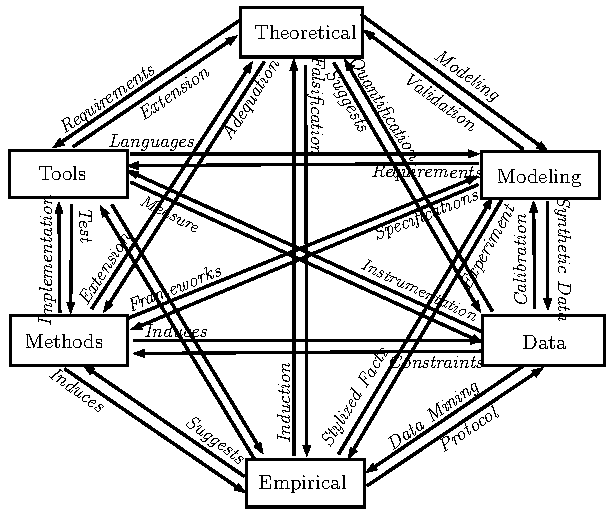
\includegraphics[width=\textwidth]{Figures/KnowledgeFramework/framework}
\caption[Full network of knowledge domains][Réseau complet des domaines de connaissance]{\textbf{Projection of a perspective into a full network of knowledge domains.} To illustrate the domains and the interaction processes between them, we do the exercise of trying to qualify all possible binary relations between two given domains. This does not reflect the real structure of the framework, but is an aid to consider what interactions can be. Note that the nature of relations is not always the same here, some being constraints, other knowledge transfer, other processes within other domains such as synthetic data which is a methodology. This shows that some domains act as catalyzers for relations between others, in this network setting, what corresponds indeed to a situation of co-evolution.
}{\textbf{Projection d'une perspective comme un réseau complet des domaines de connaissance.} Pour illustrer les domaines et les processus d'interaction possibles entre ceux-ci, nous faisons l'exercice d'essayer de qualifier toutes les relations binaires possibles entre les domaines. Cela ne reflète en rien la structure réelle du cadre, mais est une aide pour considérer ce que les interactions peuvent être. Il faut noter que la nature des relations n'est pas toujours la même ici, certaines étant des contraintes, d'autres des transferts de connaissance, d'autres processus à l'intérieur d'autres domaines comme les données synthétiques qui est une méthodologie. Cela montre que certains domaines agissent comme catalyseurs pour les relations entre les autres, dans cette configuration de réseau, ce qui correspond en fait à une situation de co-évolution.}
\label{fig:knowledgeframework:fwk}
\end{figure}
%%%%%%%%%%%%%%%%




%%%%%%%%%%%%%%%%
\subsection{Discussion}{Discussion}
%%%%%%%%%%%%%%%%



%%%%%%%%%%%%%%%%
\subsubsection{Application Range}{Portée d'application}


\bpar{
We insist that our framework does not pretend to introduce a general epistemology of scientific knowledge, but far from that is rather targeted towards reflexivity in the understanding of complex systems. The level of generality is at a very different level, but the aim to practical implication in the handling of complexity contributes to a certain generic character in applications. It is furthermore particularly suited to study Complex Systems, since more reductionist approaches can handle more compartmented production of knowledge, whereas integration of disciplines and scales and therefore domains of knowledge has been emphasized as crucial to study complexity.
}{
Nous insistons sur le fait que notre cadre ne prétend pas introduire une épistémologie générale de la connaissance scientifique, mais loin de cela est plutôt ciblé vers une réflexivité dans la compréhension des systèmes complexes. Le niveau de généralité est à niveau très différent, mais le but d'implications pratiques dans la compréhension de la complexité contribue à un certain caractère générique dans les applications. Il est de plus particulièrement adapté à l'étude des Systèmes Complexes, puisque des approches plus réductionnistes peuvent gérer des productions de connaissance plus compartimentées, tandis que l'intégration des disciplines et des échelles et donc des domaines de connaissance a été souligné comme crucial pour l'étude de la complexité.
}

%%%%%%%%%%%%%%%%
\subsubsection{Towards a formalisation}{Vers une Formalisation}


\bpar{
The knowledge framework stays at an epistemological level, and its application could be formalized in a more systematic way. We give here a possible direction to achieve that, starting from the coupling of a formalization of the system model with one of the perspective. A perspective would be defined as a dataflow machine $M$ in the sense of~\cite{golden2012modeling} that gives a convenient way to represent it and to introduce timescales and data, to which is associated an ontology $O$ in the sense of~\cite{livet2010}, i.e. a set of elements each corresponds to an entity (which can be an object, an agent, a process, etc.) of the real world. Purpose and carrier of the perspective are contained in the ontology if they make sense for studying the system. Decomposing the ontology into atomic elements $O=(O_j)_j$ and introducing an order relation between ontology elements based on weak emergence ($O_j\succcurlyeq O_i$ if and only if $O_j$ weakly emerges of $0_i$) should yield a canonical decomposition of the perspective containing the structure of the system. The challenge would be then to link this decomposition with the canonical decomposition of the dataflow machine postulated by~\cite{golden2012modeling}, and then define knowledge domains within this coupling: data is in flows of the machine, modeling in the machine, empirical and theoretical in ontologies, methods in the structure of the tree. Such an enterprise with consistent operations is however totally beyond the scope of this paper, but would be a powerful development.
}{
Le cadre de connaissances reste à un niveau épistémologique, et son application pourrait être formalisée de manière plus systématique. Pour cela, il faudrait reprendre partiellement le cadre développé dans la section précédente~\ref{sec:csframework}. Rappelons les éléments clés et comment ceux-ci peuvent s'articuler. L'aspect principal est le couplage d'une formalisation du modèle du système avec celle de la perspective. Une perspective serait définie comme une \emph{Dataflow Machine} $M$ au sens de~\cite{golden2012modeling} qui donne un moyen pratique pour la représenter et pour introduire les échelles de temps et les données, à laquelle est associée une ontologie $O$ au sens de~\cite{livet2010}, i.e. un ensemble d'éléments dont chacun correspond à une entité (qui peut être un objet, un agent, un processus, etc.) du monde réel. Le motif et l'agent porteur de la perspective sont contenus dans l'ontologie s'ils font sens pour étudier le système. Décomposer l'ontologie en éléments atomiques $O=(O_j)_j$ et introduire une relation d'ordre entre les éléments des ontologies basée sur l'émergence faible ($O_j\succcurlyeq O_i$ si et seulement si $O_j$ émerge faiblement de $0_i$) devrait fournir une décomposition canonique de la perspective contenant la structure du système. Le défi serait ensuite de lier cette décomposition avec la décomposition canonique de la \emph{Dataflow Machine} postulée par~\cite{golden2012modeling}, et ensuite définir les domaines de connaissance au sein de ce couplage : les données sont dans les flots des machines, le modèle est la machine, l'empirique et le théorique dans les ontologies, les méthodes dans la structure de l'arbre. Une telle entreprise avec des opérations cohérentes entre les éléments est cependant hors de notre portée pour l'instant, mais serait un développement puissant.
}



\bpar{
We have studied with mixed method the construction of a scientific theory in theoretical and quantitative geography, and from that inductively introduced a knowledge framework aiming at understanding the production of knowledge on complex system as a complex system itself, namely a perspective with co-evolving components within interdependent knowledge domains. Note that the approach is fully reflexive as several components were necessary. We believe our framework is a useful tool to study complexity and manage complex systems, since it explicits some choices and directions of developments that may otherwise be unconscious.
}{
Nous avons étudié par des méthodes mixtes la construction d'une théorie scientifique en géographie théorique et quantitative, et à partir de cela introduit de manière inductive un cadre de connaissances visant comprendre la production de connaissances sur un système complexe comme un système complexe elle-même, plus précisément une perspective avec des composantes co-évolutives au sein de domaines de connaissances interdépendants. On peut noter que cette approche est totalement réflexive puisque plusieurs de ces composantes ont été nécessaires. Nous postulons que ce cadre peut être un outil utile pour étudier la complexité et gérer des systèmes complexes, puisqu'il explicite certains choix et directions de développements qui pourraient autrement être inconscients.
}










%-------------------------


\subsubsection[Co-construction of theories and models][Co-construction des théories et modèles]{Co-construction of theories and models: an synthesis of our contributions}{Co-construction des théories et modèles en géographie quantitative : une synthèse de nos contributions}



Nous concluons ce chapitre d'ouverture par une mise en perspective cohérente des diverses contributions de la thèse, du point de vue de l'illustration de la co-évolution des connaissances dans différents domaines, et de boucler la boucle par un retour sur la construction de la théorie géographique. Comme précisé en préambule, un mode de lecture linéaire serait trop réducteur, puisque la plupart des travaux s'enrichissent mutuellement quel que soit leur domaine et leur portée, et un compte-rendu linéaire, au delà d'être intrinsèquement appauvrissant, est en quelque sorte un mensonge par omission de l'ensemble des interactions complexes entre les pans de connaissance produite. Bien sûr l'exercice de synthèse et la capacité à faire rentrer dans un cadre formaté imposé, sont louables, voir souhaitables dans l'état actuel des conditions de production scientifiques. Mais une posture fondamentale que nous prendrons et défendrons tout au long de ce travail est celle d'une science anarchiste proposée par \noun{Feyerabend}, qui sans être prise purement littéralement et mise en contexte, est extrêmement fructifiante pour proposer des changements de paradigmes et s'émanciper de travaux \emph{mainstream} dont les bases et la légitimité semblent s'enrichir malgré les critiques croissantes. L'écriture d'une monographie extrêmement formatée ne présente généralement que peu d'intérêt de par le caractère contraint de l'exercice (combien d'interminables chapitres ``état de l'art'' et ``problématique'' ou ``enjeux sociaux'' témoignent d'une platitude au point de vouloir arrêter la lecture d'un ouvrage par ailleurs remarquable, ce qui s'est sûrement passé dans notre cas d'ailleurs), et parait relativement vaine vu la destinée de prendre la poussière dans une étagère obscure d'un laboratoire obscur, sans être sauvé par la mise en ligne vu la langue imposée\footnote{Ce qui relève bien sûr par ailleurs d'une problématique bien plus complexe que la simple audience~\cite{tardy2004role} et la richesse des pensées scientifiques permises par l'utilisation de différentes langues n'est pas discutable ainsi que la légitimité d'organisations comme l'ASRDLF. Mais c'est bien cette audience qui nous pose problème ici et dans ce cas il est quasiment aussi vieux jeu pour une école doctorale d'imposer le français comme langue d'écriture que le discours du consul et son snobisme d'énarque rapportés en~\ref{sec:casestudies}.}. On se rêve d'imaginer une thèse entièrement digitale et dont le cheminement du lecteur tracé dans le support numérique serait à l'origine d'une multitude de visions possibles, traduisant effectivement la complexité du processus de construction, et des perspectives d'enrichissement innombrables par une rétroaction et une interaction avec les lecteurs, c'est à dire sortir du mode de présentation linéaire, comme déjà soutenu en introduction. L'invention de nouveaux modes de communication scientifiques est un défi urgent à part entière, et notre ébauche de réflexivité développée en Appendice~\ref{app:reflexivity} cherche à y contribuer.



La construction de théories géographiques, dans le cadre d'une Géographie Théorique et Quantitative, s'effectue par itérations dans une dynamique de co-évolution avec les efforts empiriques et de modélisation~\cite{livet2010}. Parmi les nombreux exemples, on peut citer la théorie évolutive des villes (co-construite par un spectre de travaux s'étendant par exemple des premières propositions de \cite{pumain1997pour} jusqu'aux résultats matures présentés dans~\cite{pumain2012multi}), l'étude du caractère fractal des structures urbaines (par exemple de \cite{frankhauser1998fractal} à \cite{frankhauser2008fractal}) ou plus récemment le projet Transmondyn visant à enrichir la notion de transition des systèmes de peuplement (ouvrage à paraître). Cette communication propose un format original en s'inscrivant dans cette lignée, par la synthèse de différents travaux empiriques et de modélisation menés conjointement avec l'élaboration d'appareils théoriques visant à mieux comprendre les relations entre territoires et réseaux de transports. L'originalité de cette contribution réside à la fois dans la synthèse de travaux très divers pourtant reliés en filigrane, et dans la proposition d'une théorie géographique spécifique s'appuyant sur cette synthèse en seconde partie.



\paragraph{}{Pourquoi une théorie et des modèles de co-évolution}


Notre première entrée prend un point de vue d'épistémologie quantitative pour tenter d'expliquer le fait que, si la co-évolution entre territoires et réseaux a par exemple été prouvée par~\cite{bretagnolle:tel-00459720}, la littérature est très pauvre en modèles de simulation endogenéisant cette co-évolution. Une exploration algorithmique de la littérature a été menée dans \cite{raimbault2015models}, suggérant un cloisonnement des domaines scientifiques s'intéressant à ce sujet. Des méthodes plus élaborées ainsi que les outils correspondants (collecte et analyse des données), couplant une analyse sémantique au réseau de citations, ont été développées pour renforcer ces conclusions préliminaires~\cite{raimbault2016indirect}, et les premiers résultats au second ordre semblent confirmer l'hypothèse d'un domaine peu défriché car à l'intersection de champs ne dialoguant pas nécessairement aisément. Ces premiers résultats d'épistémologie quantitative confirment l'intérêt d'une modélisation couplant des processus relevant de différentes échelles et domaines d'études, et surtout l'intérêt de l'élaboration d'une théorie propre.


\paragraph{}{Etudes empiriques}

Le premier axe pour les développements en eux-mêmes consiste en des analyses empiriques. Une étude des corrélations spatiales statiques entre mesures de forme urbaine (indicateurs morphologiques calculés sur la grille de population eurostat) et mesures de forme de réseau (topologie du réseau routier issu d'OpenStreetMap), sur l'ensemble de l'Europe à différentes échelles, a pu révéler la non-stationnarité et la multi-scalarité spatiale de leurs interactions~\cite{raimbault2016cautious}. Cet aspect a aussi été mis en évidence dans l'espace et le temps à une échelle microscopique lors de l'étude des dynamiques d'un système de transport~\cite{raimbault2016investigating}, conjointement avec l'hétérogénéité des processus pour un autre type de système~\cite{raimbault2015hybrid}. Ces faits stylisés valident pour l'instant l'utilisation de modèles de simulation complexes, pour lesquels des premiers efforts de modélisation ont ouvert la voie vers des modèles plus élaborés.


\paragraph{}{Modélisation}

A l'échelle mesoscopique, des processus d'agrégation-diffusion ont été prouvés suffisant pour reproduire un grand nombre de formes urbaines avec un faible nombre de paramètres, calibrés sur l'ensemble du spectre des valeurs réelles des indicateurs de forme urbaine pour l'Europe. Ce modèle simple a pu, à l'occasion d'un exercice méthodologique explorant le possibilité de contrôle au second ordre de la structure de données synthétiques~\cite{raimbault2016generation}, être couplé faiblement à un modèle de génération de réseau, démontrant une grande latitude de configurations potentiellement générées. L'exploration de différentes heuristiques autonomes de génération de réseau a par ailleurs été entamée~\cite{raimbault2015labex}, pour comparer par exemple des modèles de croissance de réseau routier basés sur l'optimisation locale à des modèles inspirés des réseaux biologiques : chacun présente une très grande variété de topologies générées. A l'échelle macroscopique, un modèle simple de croissance urbaine calibré dynamiquement sur les villes françaises de 1830 à 2000 (base Pumain-Ined) a permis de démontrer l'existence d'un effet réseau de par l'augmentation de pouvoir explicatif du modèle lors de l'ajout d'un effet des flux transitant par un réseau physique, tout en corrigeant le gain dû à l'ajout de paramètres par la construction d'un Critère d'Information d'Akaike empirique~\cite{raimbault2016models}. Cet ensemble de modèles se positionne avec un objectif de parcimonie et dans une perspective d'application en multi-modélisation. Dans une démarche basée-agent plus descriptive et donc par un modèle plus complexe, \cite{le2015modeling} décrit un modèle de co-évolution à l'échelle métropolitaine (modèle Lutecia) qui inclut en particulier des processus de gouvernance pour le développement des infrastructures de transport. Même si ce dernier modèle est toujours en exploration, les premières études de la dynamique montre l'importance du caractère multi-niveau du développement du réseau de transport pour obtenir des motifs complexes de réseaux et de collaboration entre agents. L'ensemble de ces premiers efforts de modélisation, bien qu'ils ne soient pas majoritairement centrés sur des modèles de co-évolution à proprement parler, supportent les premiers fondements théoriques que nous proposons par la suite.



\paragraph{}{Construction d'une Théorie Géographique}

Nous revoyons enfin sous l'oeil de la co-evolution des domaines la théories construite en~\ref{sec:theory}. Nous insistons ici sur son caractère intégratif permettant de joindre Théorie Evolutive et Morphogenèse. En se basant sur les travaux précédents, nous proposons de joindre deux entrées pour la construction d'une théorie géographique ayant un focus privilégié sur les interactions entre territoires et réseaux. La première est par la notion de \emph{morphogénèse}, qui a été explorée d'un point de vue interdisciplinaire dans~\cite{antelope2016interdisciplinary}. Pour notre part, la morphogenèse consiste en l'émergence de la forme et de la fonction, via des processus locaux autonomes dans un système qui exhibe alors une architecture auto-organisée. La présence d'une fonction et donc d'une architecture distingue les systèmes morphogénétiques de systèmes simplement auto-organisés (voir~\cite{doursat2012morphogenetic}). De plus, les notions d'autonomie et de localité s'appliquent bien à des systèmes territoriaux, pour lesquels on essaye d'isoler les sous-systèmes et les échelles pertinentes. Les travaux sur la génération de forme urbaine calibrée par des processus autonomes, les premiers travaux sur la génération de réseaux par de multiples processus également autonomes, et des travaux plus anciens étudiant un modèle simple de morphogenèse urbaine qui suffisait à reproduire des motifs de forme stylisés~\cite{raimbault2014hybrid}, nous suggèrent la possible existence de tels processus au sein des systèmes territoriaux. D'autre part, le cadre d'un théorie évolutive des villes est plébiscité par nos résultats empiriques, qui montrent le caractère non-stationnaire, hétérogène, multi-scalaire des systèmes urbains. Pour rester le plus général possible, et comme nos résultats à la fois empiriques et de modélisation (génération de formes quelconques par le modèle d'agrégation-diffusion par exemple) s'appliquent aux systèmes territoriaux en général, nous nous plaçons dans le cadres de territoires humains de Raffestin~\cite{raffestin1988reperes}, c'est à dire ``la conjonction d'un processus territorial avec un processus informationnel'', qui peut être interprété dans notre cas comme le système complexe socio-techno-environmental que constitue un territoire et les agents et artefacts qui y interagissent. L'importance des réseaux est soulignée par nos résultats sur la nécessité du réseau dans le modèle de croissance macroscopique : nous proposons alors de parler de \emph{Systèmes Territoriaux Complexes en Réseaux}, en ajoutant au plongement du territoire dans la théorie évolutive la particularité qu'il existe des composantes cruciales qui sont les réseaux (de transport en l'occurrence), dont l'origine peut être expliquée par la théorie territoriale des réseaux de Dupuy~\cite{dupuy1987vers}. Nous spéculons alors l'hypothèse suivante afin de réconcilier nos deux approches : \textbf{l'existence de processus morphogénétiques dans lesquels les réseaux ont un rôle crucial est équivalente à la présence de sous-systèmes dans les systèmes territoriaux complexes en réseaux, qu'on définit alors comme co-évolutifs.} Cette proposition a de multiples implications, mais a typiquement guidé notamment les choix de modélisation vers une méthodologie modulaire et de multi-modélisation afin d'essayer d'exhiber des processus morphogénétiques, ainsi que les travaux empiriques vers une étude plus poussée des correlations, causalités (dans le cas de séries temporelles) et recherche de décompositions modulaires des systèmes.



\stars






